\textbf{Motivation.} Time-to-close is a common proxy for how quickly maintainers act on an issue, and it has long been studied as a property of issues~\cite{kikas2016lifetime}. For an adopter, it answers a practical question: do the issues that come with one agent sit idle longer than those of another? It also comes with a pitfall. A third of the issues in the data are still open, and any analysis that uses only closed issues leaves out the slowest ones.

\textbf{Approach.} The first comparison uses the \NRQTwo{} closed issues of the eleven tested agents. Their time-to-close is far from normal: Shapiro--Wilk~\cite{shapiro1965normality} rejects normality for every agent (\(p < 10^{-6}\); skewness \SkewMin\ to \SkewMax), and even after a log transformation it is rejected for \NNonNormalLog{} of the eleven agents. The right tail is long: across the tested agents, the mean time-to-close is \TTCMeanAll{} hours against a median of \TTCMedianAll{} hours (IQR \TTCIQRAll{} h, SD \TTCSDAll{} h), and the Q--Q plots in the replication package show the same pattern for every agent. The comparison therefore uses the Kruskal--Wallis test with \(\varepsilon^2\), Dunn's pairwise test with Holm correction and Cliff's \(\delta\). It is then repeated on all issues of the tested agents with the Kaplan--Meier estimator, which counts an issue that is still open as censored, so that it contributes the time it has been open without being treated as closed. Finally, the main test is repeated on the four sensitivity subsets S1--S4.

\begin{table}[t]
\caption{Time-to-close per agent. Closed issues: count, median in hours with exact 95\% CI, rank. All issues: \% still open, Kaplan--Meier (KM) median in days (n.r.\ = 50\% closed never reached), rank}\label{tab:rq2}
\centering\footnotesize\setlength{\tabcolsep}{2.5pt}
\resizebox{\columnwidth}{!}{\begin{tabular}{@{}lrrcrrrr@{}}
\toprule
& \multicolumn{3}{c}{Closed issues} & \multicolumn{2}{c}{All issues} & \multicolumn{2}{c}{Rank}\\
\cmidrule(lr){2-4}\cmidrule(lr){5-6}\cmidrule(l){7-8}
Agent & n & Median & 95\% CI & Open & KM & Closed & KM\\
\midrule
\inputtab{generated/tab_rq2_ttc.tex}
\bottomrule
\end{tabular}}
\end{table}

\textbf{Results.} \emph{Closed issues.} Time-to-close differs across agents (Kruskal--Wallis \(H = \KWH\), df = \KWdf, \(p = \KWp\)) with a \KWeff{} effect (\(\varepsilon^2 = \KWeps\)). Medians range from \MedPrAgent{} hours for PR-Agent and \MedClaudeCode{} hours for Claude Code to \MedCoderabbit{} hours for CodeRabbit (Table~\ref{tab:rq2}). The overall effect, however, comes from a few agents at the extremes. Only \NSig{} of the 55 pairs of agents differ significantly after Holm correction, and by Cliff's \(\delta\), \NPairsNegligible{} pairs differ negligibly, \NPairsSmall{} slightly, \NPairsMedium{} moderately and \NPairsLarge{} strongly. The largest difference is between Claude Code and CodeRabbit (\(\delta = \DeltaMax\)), and Claude Code takes part in four of the five medium differences. The effect stays medium when issues closed as completed (\(\varepsilon^2 = \EpsCompleted\)) and issues closed as not planned (\(\varepsilon^2 = \EpsNotPlanned\), \NAgentsNotPlanned{} agents with at least ten such issues) are tested separately.

\emph{Robustness.} The effect remains medium without pre-release issues (S1, \(\varepsilon^2 = \EpsSOne\)), on the CodAGE precision subset (S3, \(\varepsilon^2 = \EpsSThree\)) and with one value per agent and repository (S4, \(\varepsilon^2 = \EpsSFour\)), so issues repeated in the same repository do not drive it. It shrinks to small when only human-authored issues are kept (S2, \(\varepsilon^2 = \EpsSTwo\)), which suggests that part of the difference between agents is associated with bot authorship. The ranking of the agents hardly changes in any subset (Spearman \(\rho \geq \RhoSTwo\)).

\begin{figure*}[t]
\centering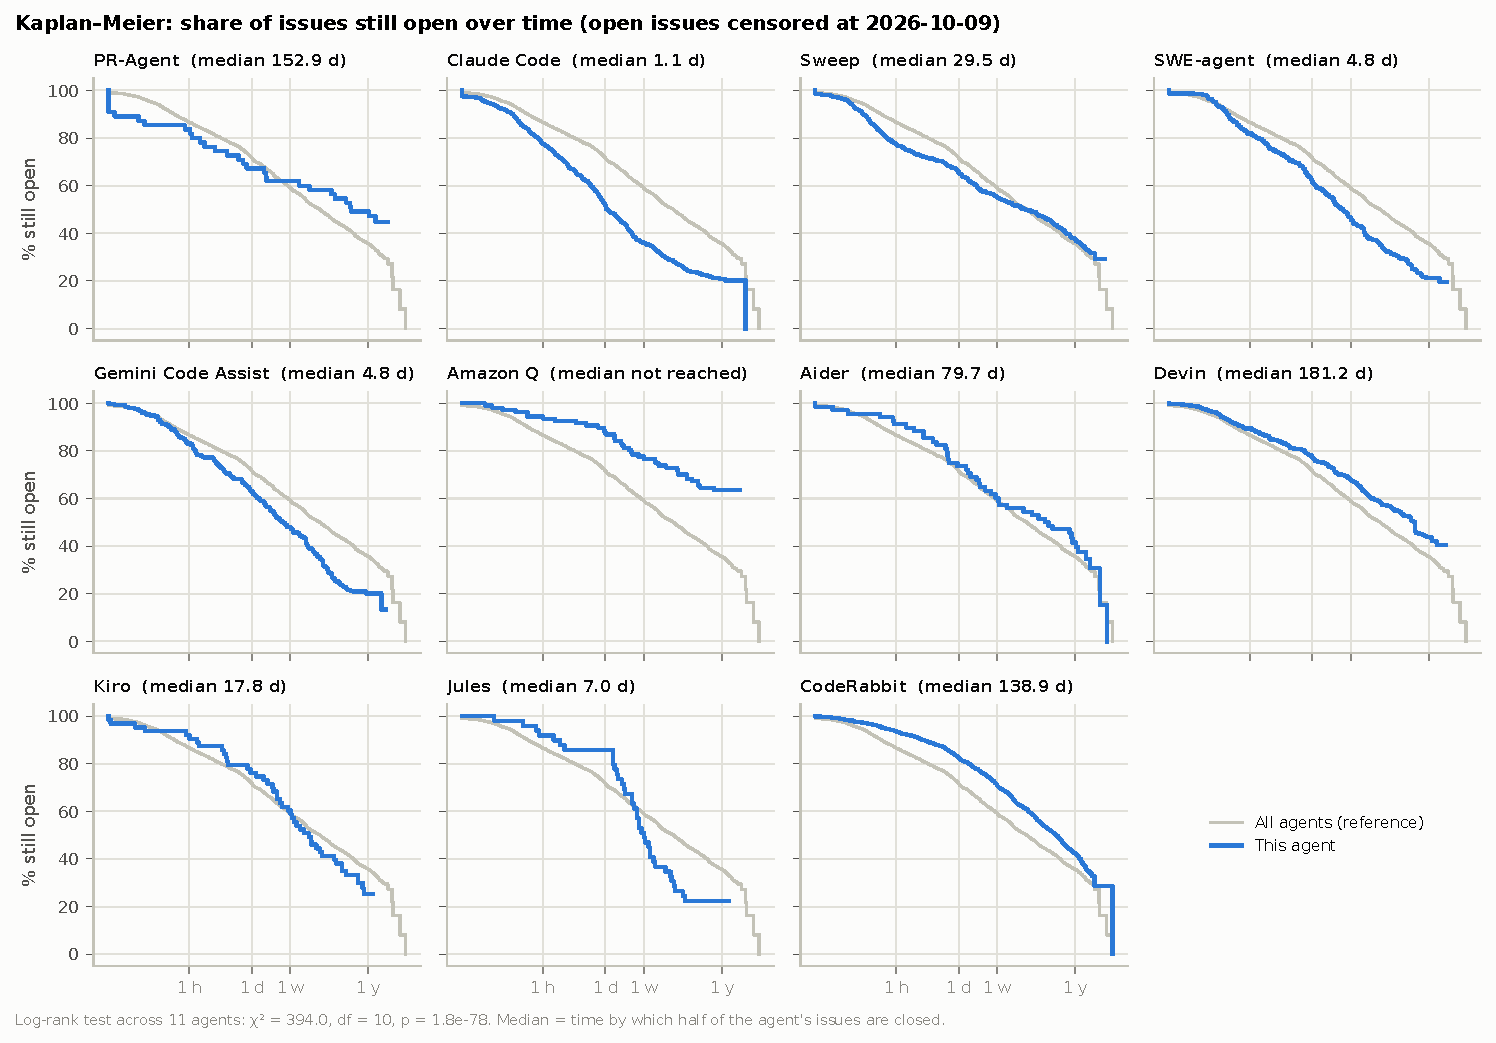
\includegraphics[width=0.86\textwidth]{rq2_R3_kaplan_meier.pdf}
\caption{Kaplan--Meier curves: share of each agent's issues still open over time, with open issues censored. The grey line shows all agents together.}\label{fig:km}
\end{figure*}

\emph{Counting the issues that are still open.} The picture changes once open issues are taken into account (Fig.~\ref{fig:km}). The difference between agents remains significant (log-rank \(\chi^2 = \LRchi\), \(p = \LRp\)), but the two rankings barely agree (Spearman \(\rho = \RankRho\)). PR-Agent, the fastest agent on closed issues, drops to 9th, because \PctOpenPrAgent\% of its issues are still open. Amazon Q falls from 6th to last: \PctOpenAmazonQ\% of its issues are open, so its Kaplan--Meier curve never reaches 50\% closed. Jules moves the other way, from 10th to 4th. Claude Code is fast under both views, 2nd on closed issues and 1st with Kaplan--Meier (median \KMClaudeCode{} days).

\emph{The role of the agent again.} The same bias affects the comparison of bot-written and other issues within an agent. Among \emph{closed} issues, bot-written CodeRabbit issues take longer than other CodeRabbit issues (median \YOwnCoderabbit{} against \YOtherCoderabbit{} hours, \(\delta = \YDeltaCoderabbit\)), but bot-written Devin issues are closed \emph{faster} than other Devin issues (\YOwnDevin{} against \YOtherDevin{} hours, \(\delta = \YDeltaDevin\)). Once open issues are counted, the bot-written issues of both agents are far slower: the Kaplan--Meier median is \YKMOwnCoderabbit{} against \YKMOtherCoderabbit{} days for CodeRabbit and \YKMOwnDevin{} against \YKMOtherDevin{} days for Devin (log-rank, Holm-adjusted \(p = \YLRpCoderabbit\) and \(\YLRpDevin\)). For Devin, then, the closed issues alone would suggest the opposite of what happens to its issues as a whole.

\rqsummary{RQ2}{Time-to-close differs across agents with a medium effect, but mostly at the extremes: 50 of the 55 pairs of agents differ negligibly or slightly. How open issues are handled changes the answer. Ranking agents by their closed issues disagrees with a survival analysis that counts open issues (\(\rho = \RankRho\)), and for Devin the closed issues alone even reverse the comparison between bot-written and other issues. Comparisons of agent speed should use survival analysis rather than closed issues only.}
